\section{C++}
\subsection{C++ template}
\raggedbottom\lstinputlisting[style=cpp]{code/c++/template.cpp}
\hrulefill
\subsection{Opcion}
\raggedbottom\lstinputlisting[style=cpp]{code/c++/alternativa.cpp}
\hrulefill
\subsection{Comand to compare output}
\subsubsection{Linux}
\raggedbottom\lstinputlisting[style=cpp]{code/c++/compare_output_linux.bash}
\subsubsection{windows}
\raggedbottom\lstinputlisting[style=cpp]{code/c++/compare_output_windows.cmd}

\hrulefill
\subsection{Bits Manipulation}
\hrulefill

\subsection{Custom Hash}
\raggedbottom\lstinputlisting[style=cpp]{code/c++/custom_hash.cpp}
\hrulefill
\subsection{Trie}
\raggedbottom\lstinputlisting[style=cpp]{code/strings/trie.cpp}
\hrulefill
\subsection{Suffix Tree}
\raggedbottom\lstinputlisting[style=cpp]{code/strings/suffix_tree.cpp}
\hrulefill

\section{Graph algorithms}
\subsection{DFS cpbook}
\raggedbottom\lstinputlisting[style=cpp]{code/graph/dfs_cpbook.cpp}
\hrulefill
\subsection{DFS iterativo - Lucas}
\raggedbottom\lstinputlisting[style=cpp]{code/graph/dfs_iterativo_Lucas.cpp}
\hrulefill
\subsection{BFS cpbook}
\raggedbottom\lstinputlisting[style=cpp]{code/graph/bfs_cpbook.cpp}
\hrulefill

\subsection{BFS para camino mas corto de UN nodo a todos los DEMAS}
\raggedbottom\lstinputlisting[style=cpp]{code/graph/bfs_camino_mas_corto.cpp}
\hrulefill

\subsection{BFS bipartito}
\raggedbottom\lstinputlisting[style=cpp]{code/graph/bfs_bipartito.cpp}
\hrulefill

\subsection{DFS detect cycle}
\raggedbottom\lstinputlisting[style=cpp]{code/graph/dfs_detect_cycles.cpp}
\hrulefill

\subsection{Dijkstra camino mas corto grafo dirigido CON PESOS(O((V+E)log V))}
\raggedbottom\lstinputlisting[style=cpp]{code/graph/dijkstraLucas.cpp}
\hrulefill
\section{Data Structures}
\subsection{unordered\_map\textless clave,valor\textgreater (hacer siempre RESERVE)}
Almacena pares clave valor.
\begin{verbatim}
unordered\_map<int,int> a;
a.reserve(n*1.33); IMPORTANTEEEEEEE
n = 1e6 aprox 42.6 MB

n = 3e6 aprox 128 MB

n = 5e6 aprox 213 MB (aún puede entrar, pero ojo con pila
, I/O buffers, otros contenedores).
\end{verbatim}

\subsubsection{Ejemplo basico Contar frecuencias}
\raggedbottom\lstinputlisting[style=cpp]{code/data-structures/unordered_map/contar_frecuencias.cpp}
\hrulefill
\subsubsection{Buscar existencia de una llave}
\raggedbottom\lstinputlisting[style=cpp]{code/data-structures/unordered_map/existencia_llave.cpp}
\hrulefill
\subsubsection{Transformar indices dispersos a continuos}
\raggedbottom\lstinputlisting[style=cpp]{code/data-structures/unordered_map/comprimir_indices.cpp}
\hrulefill
\subsubsection{Hashing pair}
\raggedbottom\lstinputlisting[style=cpp]{code/data-structures/unordered_map/hashing_pair.cpp}
\hrulefill
\subsection{unordered\_set\textless clave\textgreater (hacer siempre RESERVE)}
\begin{verbatim}
No existe acceso aleatorio con h[] ,
pero se puede iterar con for auto.
\end{verbatim}
\raggedbottom\lstinputlisting[style=cpp]{code/data-structures/unordered_set/ejemplo_basico.cpp}
\hrulefill

\subsection{unordered\_multimap\textless clave,valorES\textgreater (hacer siempre RESERVE)}
\begin{verbatim}
Una misma clave puede tener varios valores asociados
\end{verbatim}
\subsubsection{Ejemplo basico}
\raggedbottom\lstinputlisting[style=cpp]{code/data-structures/unordered_multimap/ejemplo_basico.cpp}
\hrulefill
\subsubsection{Buscar por clave}
\raggedbottom\lstinputlisting[style=cpp]{code/data-structures/unordered_multimap/buscar_por_clave.cpp}
\hrulefill
\subsubsection{Delete}
\raggedbottom\lstinputlisting[style=cpp]{code/data-structures/unordered_multimap/delete.cpp}
\hrulefill

\subsection{Disjoint Set Union}
\paragraph{}
Cada que unimos dos Sets del mismo RANK(altura subgrafo, rank=4, size=16) nuestro rank aumenta en +1.Entonces para formar un RANK r se necesitan por lo menos $2^r$ vertices.
\begin{figure}[H]
    \centering
    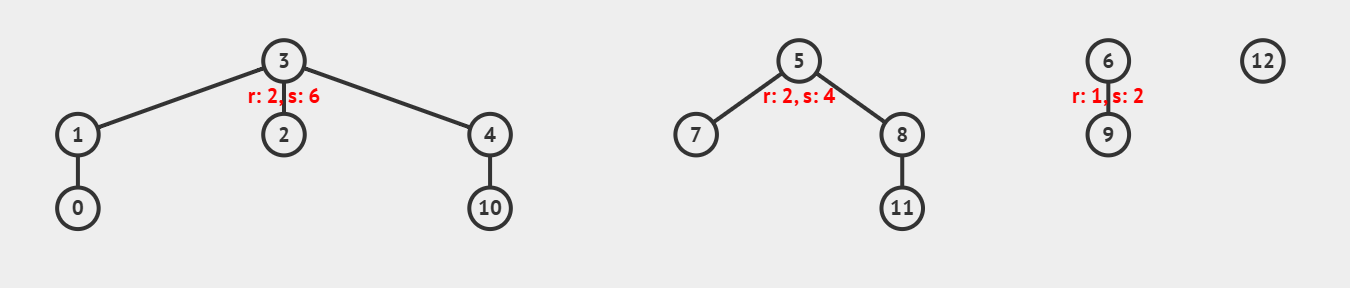
\includegraphics[width=\columnwidth]{code/pictures/UniondFind1.png}
    \caption{Inicializacion de Union-Find. Cada nodo es su propio padre.}
\end{figure}
\begin{figure}[H]
    \centering
    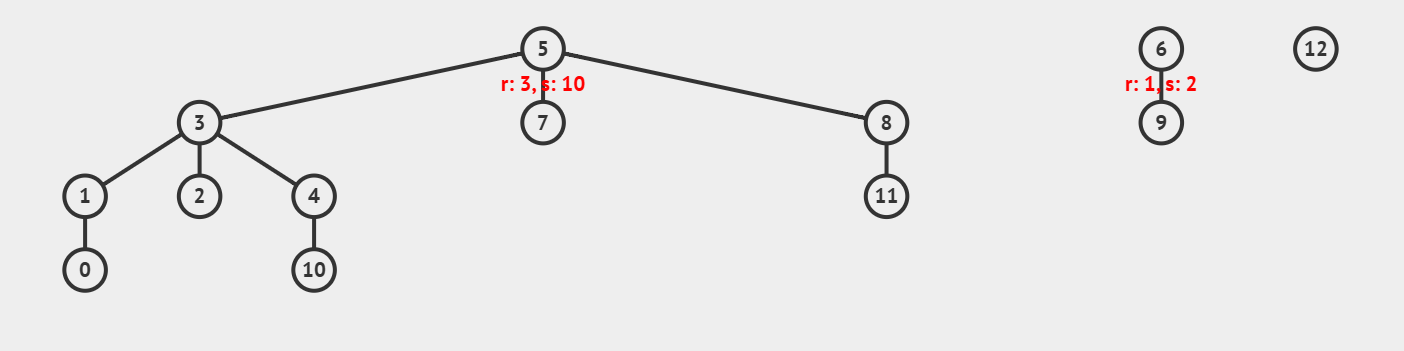
\includegraphics[width=\columnwidth]{code/pictures/UniondFind2.png}
    \caption{Union-Find despues de unir 3 y 5}
\end{figure}
\raggedbottom\lstinputlisting[style=cpp]{code/data-structures/Uniond_find_Disjoint_cpbook.cpp}
\hrulefill

\subsection{Fenwick Tree}
\raggedbottom\lstinputlisting[style=cpp]{code/data-structures/fenwick_cpbook.cpp}
\hrulefill

\subsection{Segment Tree}
\raggedbottom\lstinputlisting[style=cpp]{code/data-structures/segment_tree_cpbook.cpp}
\hrulefill

\subsection{Order Statistics Tree}
\subsubsection{Quick Selct}
\begin{verbatim}
Ranking(v) = posicion del elemento v si el 
arreglo estuviese ordenado.
\end{verbatim}
\raggedbottom\lstinputlisting[style=cpp]{code/data-structures/quickSelect.cpp}
\hrulefill
\subsection{Ordered Statistics Tree}
\raggedbottom\lstinputlisting[style=cpp]{code/data-structures/order_statistics_tree_cpbook.cpp}
\hrulefill

\section{Math}
\subsection{Prime Numbers 1-2000}
\begin{verbatim}
2 3 5 7 11 13 17 19 23 29
31 37 41 43 47 53 59 61 67 71
73 79 83 89 97 101 103 107 109 113
127 131 137 139 149 151 157 163 167 173
179 181 191 193 197 199 211 223 227 229
233 239 241 251 257 263 269 271 277 281
283 293 307 311 313 317 331 337 347 349
353 359 367 373 379 383 389 397 401 409
419 421 431 433 439 443 449 457 461 463
467 479 487 491 499 503 509 521 523 541
547 557 563 569 571 577 587 593 599 601
607 613 617 619 631 641 643 647 653 659
661 673 677 683 691 701 709 719 727 733
739 743 751 757 761 769 773 787 797 809
811 821 823 827 829 839 853 857 859 863
877 881 883 887 907 911 919 929 937 941
947 953 967 971 977 983 991 997 1009 1013
1019 1021 1031 1033 1039 1049 1051 1061 1063 1069
1087 1091 1093 1097 1103 1109 1117 1123 1129 1151
1153 1163 1167 1181 1187 1193 1201 1213 1217 1223
1229 1231 1237 1249 1259 1277 1279 1283 1289 1291
1297 1301 1303 1307 1319 1321 1327 1361 1367 1373
1381 1399 1409 1423 1427 1429 1433 1439 1447 1451
1453 1459 1471 1481 1483 1487 1489 1493 1499 1511
1523 1531 1543 1549 1553 1559 1567 1571 1579 1583
1597 1601 1607 1609 1613 1619 1621 1627 1637 1657
1663 1667 1669 1693 1699 1709 1721 1723 1733
1741 1747 1753 1759 1777 1783 1787 1789 1801 1811
1823 1831 1847 1861 1867 1871 1873 1877 1879 1889
1901 1907 1913 1931 1933 1949 1951 1973 1979 1987

 970'997 971'483 921'281'269 999'279'733
 1'000'000'009 1'000'000'021 1'000'000'409 
 1'005'012'527
\end{verbatim}
\hrulefill
\subsection{Serie de Fibonacci (hasta n=20)}
\begin{verbatim}
Def: F(0)=0  ,  F(1)=1  ,   F(n)=F(n-1)+F(n-2)
F(0) = 0
F(1) = 1
F(2) = 1
F(3) = 2
F(4) = 3
F(5) = 5
F(6) = 8
F(7) = 13
F(8) = 21
F(9) = 34
F(10) = 55
F(11) = 89
F(12) = 144
F(13) = 233
F(14) = 377
F(15) = 610
F(16) = 987
F(17) = 1597
F(18) = 2584
F(19) = 4181
F(20) = 6765
\end{verbatim}
\hrulefill
\subsection{Factorial (hasta n=20)}
\begin{verbatim}
Def: n!=n(n-1)!
0! = 1
1! = 1
2! = 2
3! = 6
4! = 24
5! = 120
6! = 720
7! = 5040
8! = 40320
9! = 362880
10! = 3628800
11! = 39916800
12! = 479001600
13! = 6227020800
14! = 87178291200
15! = 1307674368000
16! = 20922789888000
17! = 355687428096000
18! = 6402373705728000
19! = 121645100408832000
20! = 2432902008176640000
\end{verbatim}
\hrulefill
\subsection{Numeros Triangulares (hasta n=20)}
\begin{verbatim}
Def: T(n)=n(n+1)/2

T(1) = 1
T(2) = 3
T(3) = 6
T(4) = 10
T(5) = 15
T(6) = 21
T(7) = 28
T(8) = 36
T(9) = 45
T(10) = 55
T(11) = 66
T(12) = 78
T(13) = 91
T(14) = 105
T(15) = 120
T(16) = 136
T(17) = 153
T(18) = 171
T(19) = 190
T(20) = 210
\end{verbatim}
\hrulefill
\subsection{Numeros Cuadrados (hasta n=20)}
\begin{verbatim}
Def: Q(n)=n^2

Q(1) = 1
Q(2) = 4
Q(3) = 9
Q(4) = 16
Q(5) = 25
Q(6) = 36
Q(7) = 49
Q(8) = 64
Q(9) = 81
Q(10) = 100
Q(11) = 121
Q(12) = 144
Q(13) = 169
Q(14) = 196
Q(15) = 225
Q(16) = 256
Q(17) = 289
Q(18) = 324
Q(19) = 361
Q(20) = 400
\end{verbatim}
\hrulefill
\subsection{Simple Sieve of Eratosthenes O(n*log(log(n))) - con n=1e7 1.25 MB}
\raggedbottom\lstinputlisting[style=cpp]{code/math/simple_sieve_eratosthenes.cpp}
\hrulefill
\subsection{Smallest Prime Factor AND Sieve of Eratosthenes O(n) - con n=1e7 45 MB}
\raggedbottom\lstinputlisting[style=cpp]{code/math/spf_sieve_eratosthenes.cpp}
\hrulefill
\subsection{Smallest Prime Factor Piton++}
\raggedbottom\lstinputlisting[style=cpp]{code/math/spf_sieve_eratosthenes.cpp}
\hrulefill
\subsection{Combinatorics}
\subsubsection{Next permutation}
\raggedbottom\lstinputlisting[style=cpp]{code/math/spf_sieve_eratosthenes.cpp}
\hrulefill
\section{Dynamic Programming}
\section{Miscellaneous}
\subsection{Ternary Search}
\hrulefill

